\section{DESENVOLVIMENTO DA APLICAÇÃO}

Este capítulo explora o processo de criação do sistema de comunicação
com criptografia de ponta a ponta, abrangendo desde a estruturação do
ambiente técnico até os procedimentos metodológicos aplicados durante
a implementação. Apresentam-se as problemáticas identificadas no
curso do desenvolvimento e as medidas adotadas para resolvê-las,
complementado por uma visão ampla das funcionalidades implementadas e
das ferramentas tecnológicas selecionadas para o projeto.

\subsection{Contextualização e Escopo da Implementação}

A necessidade de desenvolver um sistema de comunicação
verdadeiramente seguro emerge da análise dos problemas identificados
no contexto atual da comunicação digital. Conforme evidenciado no
levantamento bibliográfico apresentado no Capítulo 2, os sistemas
convencionais de mensagens instantâneas frequentemente falham em
garantir a privacidade absoluta dos usuários, seja por questões
arquiteturais ou por modelos de negócio que dependem da análise de dados.

O desenvolvimento da solução foi orientado pela necessidade de criar
um sistema de comunicação seguro que garantisse a privacidade das
mensagens sem depender de infraestruturas centralizadas de terceiros.
A implementação resultou em dois componentes principais: um servidor
intermediário para roteamento de conexões e uma aplicação cliente
desktop para interface com o usuário.

O sistema desenvolvido endereça especificamente os seguintes aspectos
identificados na análise do problema:

\begin{itemize}
  \item Eliminação de pontos centrais de acesso ao conteúdo das mensagens;
  \item Implementação de criptografia robusta no lado cliente;
  \item Simplificação da experiência do usuário para adoção por
    não-especialistas;
  \item Transparência através de código fonte aberto para auditoria.
\end{itemize}

\subsection{Arquitetura Implementada}

A arquitetura desenvolvida seguiu o modelo cliente-servidor com
criptografia de ponta a ponta, onde o servidor atua exclusivamente
como facilitador de conexões sem acesso ao conteúdo das mensagens,
este por sua vez pode ser hospedado por usuários voluntários e não
necessariamente pelos desenvolvedores ou mantenedores.

\subsection{\textit{Back-end}}

O \textit{back-end} é responsável por aceitar as conexões Websocket vindas dos
clientes (\acsp{APP}) compatíveis com o servidor e realizar o
encaminhamento de mensagens entre os usuários, garantindo a
confidencialidade das comunicações, de modo que uma mensagem recebida
é encaminhada diretamente para o usuário de destino sem ter seu
conteúdo acessado pelo servidor. Além disso o servidor fornece uma
interface intercambiável entre clientes, podendo ser desenvolvidos
diversos aplicativos clientes diferentes entre si, porém compatíveis
com o mesmo servidor.

O \textit{back-end} foi desenvolvido totalmente em Python utilizando o FastAPI
(framework que auxilia no desenvolvimento de \acsp{API} web), o
qual, ao ser executado, fornece uma \acs{API} acessível através de uma \acs{URL}
específica para aplicativos clientes acessarem suas funcionalidades.
A estrutura do projeto do servidor ficou da seguinte forma:

\begin{figure}[H]
  \centering
  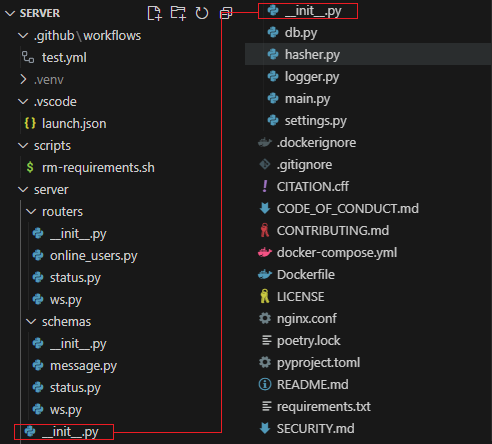
\includegraphics[width=0.6\linewidth]{imagens/estrutura-projeto-servidor.png}
  \caption[Estrutura do projeto ao fim da (numero) sprint]{Estrutura
  do projeto ao fim da (numero) sprint.}
  \label{fig:estrutura-projeto-servidor}
\end{figure}

Outro ponto importante é que neste momento já foram adicionadas
algumas dependências ao projeto que facilitaram o desenvolvimento,
entre elas, é válido destacar as seguintes:

\begin{itemize}
  \item \textit{psutil}: Biblioteca utilizada para obter informações
    sobre os recursos do hardware no qual o servidor está sendo executado;
  \item \textit{redis}: Biblioteca para gerenciamento de banco de
    dados de cache.
\end{itemize}

\subsubsection{\textit{Endpoints}}

No diretório routers ficam localizadas as definições das regras de
negócio do servidor, a maneira como ele recebe a mensagens e as
retransmite para os demais usuários, na pasta routers temos os
seguintes arquivos:

\begin{itemize}
  \item \texttt{online\_users.py}: Define um endpoint \acs{HTTP} que
    verifica se um determinado nome de usuário está disponível para
    uso, ou seja, se não há nenhum usuário online no momento que
    esteja utilizando este nome de usuário. Caso o nome de usuário
    esteja disponível a resposta \acs{HTTP} terá um código de status 200,
    caso contrário terá um código de status 409. Dessa forma, o
    código garante a integridade dos nomes de usuário ativos,
    evitando duplicidade e eventuais erros devido a conflitos de
    nomes de usuários;
  \item \texttt{status.py}: Define um endpoint \acs{HTTP} que retorna
    informações sobre o status dos recursos da máquina em que o
    servidor está sendo executado, como o uso da \acs{CPU}, frequência dos
    processadores, uso da memória, entre outras coisas;
  \item \texttt{ws.py}: Módulo principal do servidor, onde é definido
    o endpoint Websocket que trata todas as comunicações que chegam e
    saem do servidor. A rota definida aqui realiza tarefas cruciais
    para o funcionamento de todo o sistema, como armazenamento de
    conexões, usuários online, túneis de comunicação ativos,
    retransmissão de mensagens, entre outras tarefas.
\end{itemize}

\subsubsection{Esquemas de validação de dados}

Para realizar a validação de dados que entram e saem do servidor por
meio de requisições em seus endpoints \acs{HTTP} utilizamos a biblioteca
Pydantic que oferecem modelos de validação robustos e que se integram
perfeitamente com \acsp{API} \acs{JSON}, esses modelos são chamados
de \textit{schemas}.

O diretório \texttt{schemas} tem como finalidade, centralizar e gerenciar
os modelos de dados utilizados pelos \textit{endpoints} \acs{HTTP} do servidor.
Ela atua como um acordo técnico padronizado sobre os tipos de dados
que devem ser enviados e/ou recebidos entre quem realiza uma requisição a
determinado endpoint \acs{HTTP} e o servidor, garantindo validação,
consistência, segurança e documentação automática por meio do FastAPI.

Nos apêndices, o trecho de código em
"\nameref{schema:codigo-schema-status}", define alguns dos schemas de
dados usados
pelo FastAPI com o Pydantic no servidor. No fim deste arquivo, na
seção de Apêndice, os schemas desenvolvidos até este ponto estão disponíveis.

\subsubsection{Banco de dados em memória}

No sistema desenvolvido, existe a necessidade de controlar quais
usuários estão conectados em tempo real. Esse controle é fundamental
para evitar que o mesmo usuário estabeleça múltiplas sessões
simultâneas e para possibilitar a correta entrega de mensagens entre
os pares conectados. Como essas informações são voláteis e
temporárias, válidas apenas enquanto a conexão permanece ativa, não
se justifica armazená-las em um banco de dados relacional
tradicional, que implicaria em maior consumo de recursos e
complexidade desnecessária.

Diante disso, optamos pelo uso do Redis, um banco de dados NoSQL em
memória, projetado para lidar com informações temporárias de forma
rápida, leve e eficiente. Sua estrutura baseada em conjuntos permite
verificar de forma imediata se um usuário está online, além de
simplificar as operações de inserção e remoção. Dessa forma, o Redis
atendeu plenamente aos requisitos de baixa latência, simplicidade e
desempenho em tempo real exigidos pelo sistema.

O trecho de código abaixo cria uma conexão assíncrona global com o
Redis. usando configurações externas, Isso permite que qualquer parte
do sistema, como a autenticação, o Websocket, o cache, utilize o
mesmo cliente para ler e gravar dados.

O cliente Redis é utilizado principalmente no endpoint Websocket da
aplicação, para realizar o registro e exclusão de usuários que estão
online ou que se desconectaram, respectivamente. Os \acsp{ID} dos usuários
não são salvos em texto claro no Redis, mas sim um hash dos \acsp{ID}, para
garantir uma maior privacidade dos usuários. Na seção de Apêndice, em
“Código da função de hash de IDs”, está disponível o código da função
que converte qualquer \acs{ID} de usuário em um hash SHA-256, hash esse que
será usado pelo servidor para armazenamento e identificação do
usuário até o fim de sua conexão.

\subsubsection{Execução via Docker}

A execução do servidor está configurada podendo ser executada via
docker compose, garantindo que todos os serviços dos quais o servidor
depende sejam iniciados simultaneamente. Os três containers iniciados
via docker compose são os seguintes:

\begin{itemize}
  \item Redis - como banco de dados em memória;
  \item Servidor de aplicação FastAPI;
  \item Servidor web Nginx - atua como proxy reverso, recebendo as
    requisições externas e encaminhando-as para o servidor FastAPI.
\end{itemize}

O arquivo \texttt{docker-compose.yml} define três containers que compõem a
arquitetura da aplicação. O primeiro é o \textit{server}, responsável por
executar a aplicação FastAPI. Esse container é construído a partir do
código-fonte local, recebe as variáveis de ambiente necessárias para
se conectar ao Redis e está configurado para reiniciar
automaticamente em caso de falhas. Além disso, ele monta o diretório
do projeto dentro do container, permitindo que o código seja
atualizado sem necessidade de reconstrução da imagem, e estabelece
dependência direta do serviço Redis, garantindo que o banco de dados
em memória esteja disponível antes de sua inicialização.

O segundo container é o \textit{web}, que executa o servidor Nginx na
função de proxy reverso. Ele expõe a aplicação externamente através
da porta 9000 do host, redirecionando as requisições para o servidor
FastAPI. O Nginx é configurado por meio de um arquivo de configuração
customizado (\texttt{nginx.conf}), o que possibilita definir regras
específicas para o encaminhamento das requisições e otimizações de
desempenho. Assim como o servidor de aplicação, esse container também
está configurado para reiniciar automaticamente e depende do serviço
\texttt{server}, de forma que só inicia após a aplicação estar em funcionamento.

O terceiro container é o \textit{redis}, que fornece o banco de dados em
memória utilizado pela aplicação para armazenamento temporário e
operações de alta performance. Ele é baseado na imagem oficial do
Redis em sua versão otimizada \texttt{alpine}, expõe a porta 6379 para
permitir a comunicação entre os serviços e mantém a persistência dos
dados em um volume chamado \texttt{redis\_data}, evitando perda de
informações em reinicializações. Esse container também está
configurado para reiniciar automaticamente, assegurando sua
disponibilidade contínua durante a execução do sistema.

\newpage
